\documentclass{beamer}
\usepackage{xcolor}
\usetheme{Rochester}
\usecolortheme{beaver}
\AtBeginSection[]
{
  \begin{frame}
    \frametitle{Table of Contents}
    \tableofcontents[
    sectionstyle=show/shaded,
    subsectionstyle=show/show/shaded,
    subsubsectionstyle=show/show/show/shaded
    ]
  \end{frame}
}
% Frame title count
\newcounter{cont_frame}
\makeatletter
\setlength{\parindent}{0pt}
\setbeamertemplate{frametitle continuation}{%
    \setcounter{cont_frame}{\beamer@endpageofframe}%
    \addtocounter{cont_frame}{1}%
    \addtocounter{cont_frame}{-\beamer@startpageofframe}%
    (\insertcontinuationcount/\arabic{cont_frame})%
}
\makeatother
% Frame number in right down corner
\setbeamertemplate{sidebar right}{}
\setbeamertemplate{footline}{%
\hfill\usebeamertemplate***{navigation symbols}
\hspace{1cm}\insertframenumber{}/\inserttotalframenumber}


\title{LSH}
\begin{document}
	\maketitle
	\section{Review of LSH Search Scheme}
	\subsection{Multi-Probe LSH}
\begin{frame}
\frametitle{The Idea of Multi-Probe LSH~\cite{lv2007multi}}
Trade time for space:\\
Reduce the number of hash table while achieving similar performance by probing a sequence of buckets in one hash table.

\begin{table}
\begin{tabular}{|c|c|}
\hline
  \textbf{Scheme} & \textbf{Query}\\ \hline
  Basic& $g(q)=(h_1(q), h_2(q), ..., h_M(q))$ \\ \hline
  Multi-Probe& $g(q){+}\Delta^{(i)}, i{=}1,2,...,T$, $\Delta^{(i)}{=}(\delta_1^{(i)}, \delta_2^{(i)}, ..., \delta_M^{(i)})$ \\ \hline
\end{tabular}
\end{table}
\end{frame}

\begin{frame}[shrink]
	\frametitle{Probing Sequence}
	\begin{itemize}
		\item Step-Wise: \\
		Firstly search all 1-step perturbations, then 2-step ones, and so on.
		The total number of all $n$-step buckets is $L{\times} {M\choose n}{\times}2^n$.
		\item Query Based: \\
		$h(q)=\lfloor\frac{a\cdot q+b}{W}\rfloor$, $f(q)=a\cdot q + b$,\\ $f(p)-f(q)$ follows Gaussian distribution.\\
		$P(h(p)=h(q)+\Delta)\approx C\exp(\sum_{i=1}^{T}x_i(\delta_i)^2)$
	\end{itemize}
	\begin{figure}[h]
	\centering
	\begin{subfigure}{0.25\textwidth}
  	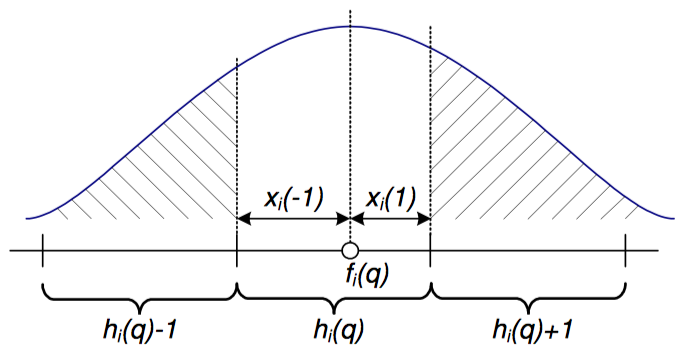
\includegraphics[width=\linewidth]{figures/multi_probe_nn}
  	\end{subfigure}
  	\begin{subfigure}{0.6\textwidth}
  	Algorithm:
  	\begin{itemize}
  		\item Sort all $x_i(-1), x_i(+1), i{=}1,2...,M$ 
  		\item Find $T$ smallest valid subset
  	\end{itemize}
  	\end{subfigure}
	\end{figure}
	
\end{frame}

\begin{frame}
\frametitle{Optimized Probing Sequence Construction}	
The perturbations sequence generated every query time.\\
Actually a certain sequence can be precomputed.\\
~\\

The idea is use $\mathbb{E}[z_j^2]$ to replace $z_j$.
$z_j$ is the $j$-th value in the sorted $x_i(\delta)$ sequence.
It can be proved that $E[z_j]{=}\frac{j}{2(M+1)}W, E[z_j^2]{=}\frac{j(j+1)}{4(M+1)(M+2)}W^2$
~\\
\end{frame}


	\subsection{Dynamic Conllision Counting}
\end{document}